\documentclass[border=15pt, multi, tikz]{article}
\usepackage{amssymb}
\usepackage[backend=bibtex,style=authoryear,natbib=true]{biblatex} % Use the bibtex backend with the authoryear citation style (which resembles APA)

\addbibresource{example.bib} % The filename of the bibliography

\usepackage[autostyle=true]{csquotes} % Required to generate language-dependent quotes in the bibliography
\usepackage{import}
\usepackage{tikz}
\usepackage{tikz-network}
\usetikzlibrary{calc,patterns,angles,quotes}
\usepackage{breqn}
\usepackage{bm}
\usepackage{graphicx}
\usepackage{subcaption}
\usepackage{multirow}
\usepackage{graphicx}
\usepackage{rotating}
\usetikzlibrary{fit}
\usetikzlibrary {arrows.meta,graphs,shapes.misc}
\usetikzlibrary {positioning}
\subimport{./layers/}{init}
\newcommand{\bn}{\textbf{n}}
\newcommand{\tabhead}[1]{\textbf{#1}}

\def\ConvColor{rgb:yellow,5;red,2.5;white,5}
\def\ConvReluColor{rgb:yellow,5;red,5;white,5}
\def\PoolColor{rgb:red,1;black,0.3}
\def\DcnvColor{rgb:blue,5;green,2.5;white,5}
\def\SoftmaxColor{rgb:magenta,5;black,7}
\def\SumColor{rgb:blue,5;green,15}
\def\poolsep{1}


\begin{document}
	
	
	
\section{Guided Gated Convolution Neural Network for Normal Inference }

\subsection{Light Net Evaluation}

We evaluate the GCNN architecture based light net on the test dataset. The light net parameters are further used as the initial parameter of light branch of the Trignet.

A qualitative evaluation of light net is shown in Figure \ref{fig:eval-light}. The average angular error are lower than $ 0.3 $ degree on all of test cases. In this case, to distinguish the output and the ground truth is already not easily only use naked eyes. 


\begin{figure}[th]
	\centering
	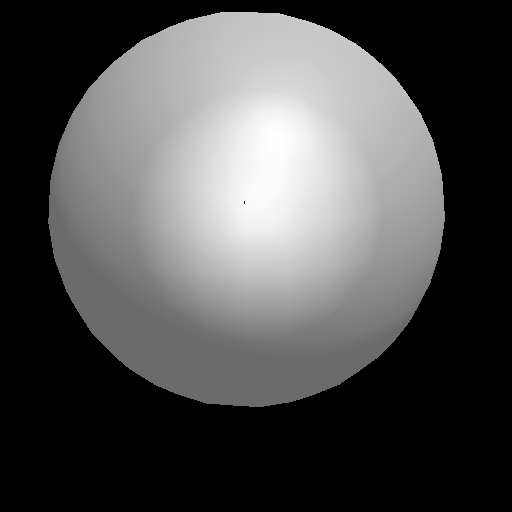
\includegraphics[width=0.18\linewidth]{./Figures/light-synthetic/fancy_eval_0_img.png}
	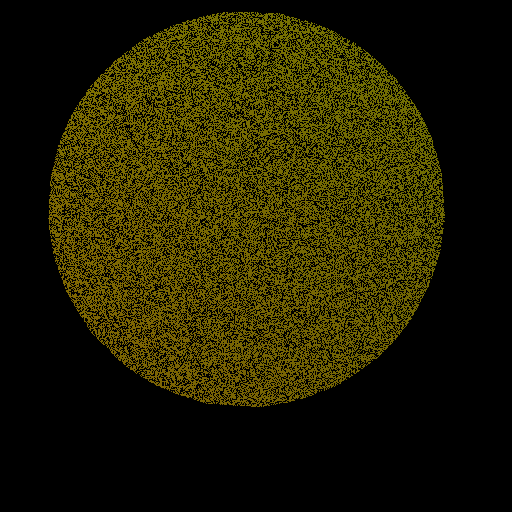
\includegraphics[width=0.18\linewidth]{./Figures/light-synthetic/fancy_eval_0_light_input.png}
	
\includegraphics[width=0.18\linewidth]{./Figures/light-synthetic/fancy_eval_0_light_light.png}
	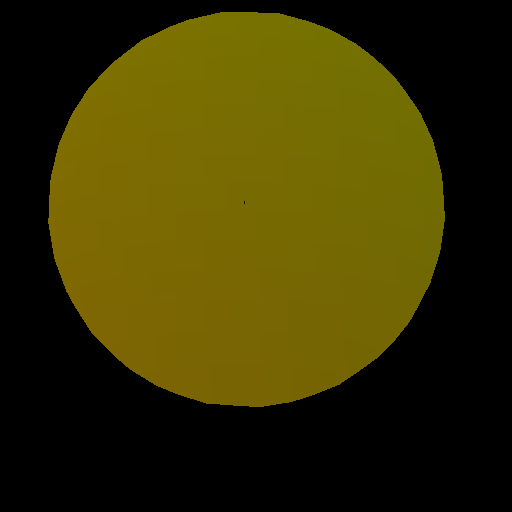
\includegraphics[width=0.18\linewidth]{./Figures/light-synthetic/fancy_eval_0_light_gt.png}
	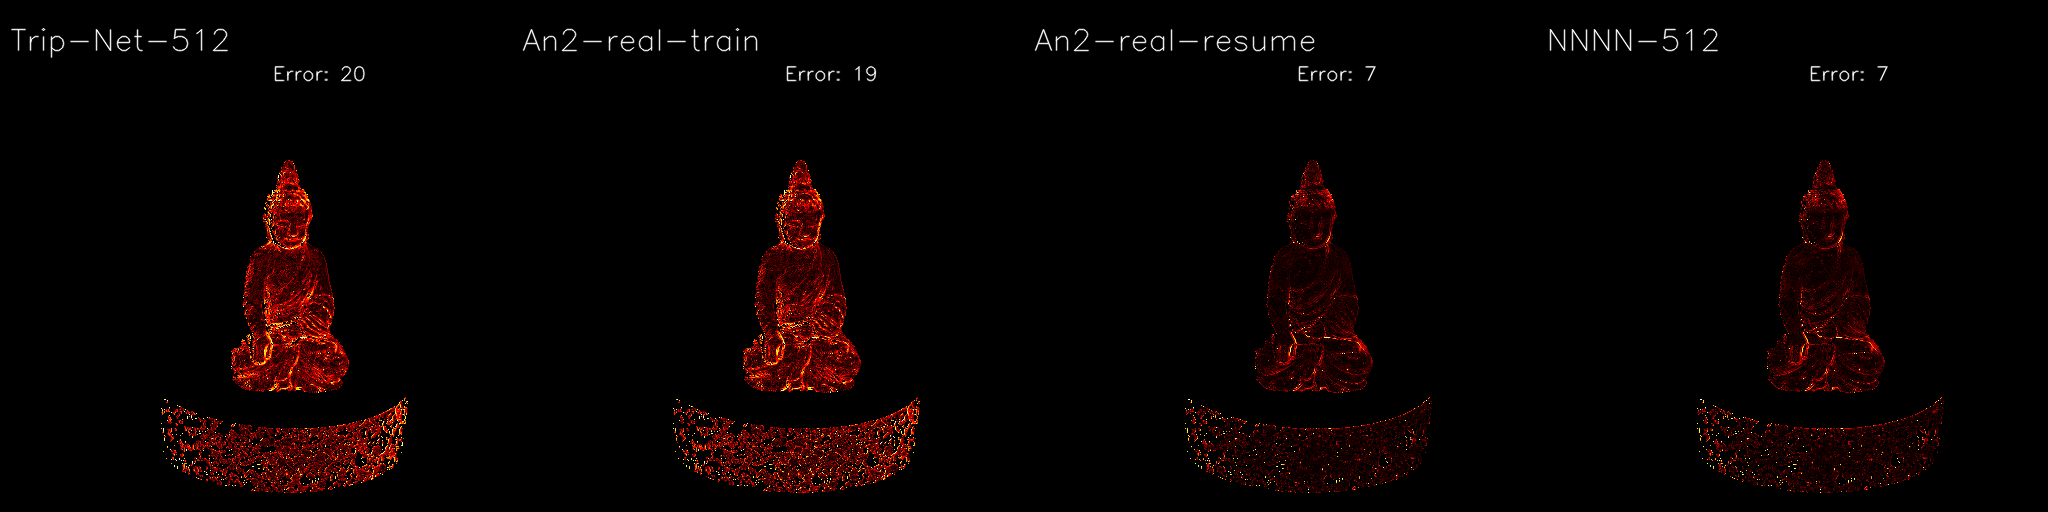
\includegraphics[width=0.18\linewidth]{./Figures/light-synthetic/fancy_eval_0_output_error.png}
	
	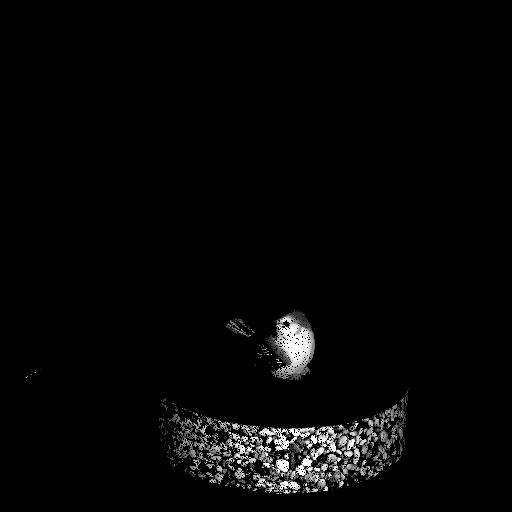
\includegraphics[width=0.18\linewidth]{./Figures/light-synthetic/fancy_eval_1_img.png}
	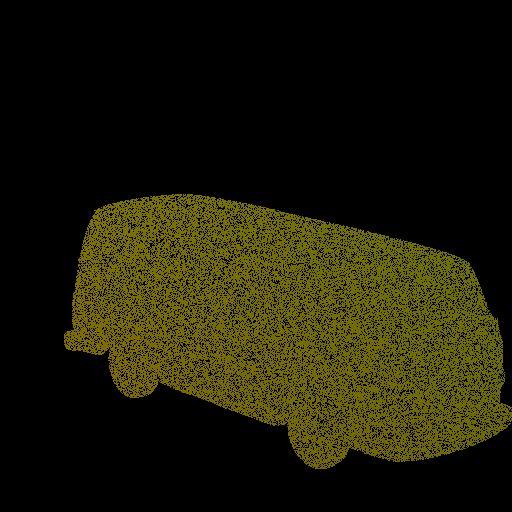
\includegraphics[width=0.18\linewidth]{./Figures/light-synthetic/fancy_eval_1_light_input.png}
	
\includegraphics[width=0.18\linewidth]{./Figures/light-synthetic/fancy_eval_1_light_light.png}
	
\includegraphics[width=0.18\linewidth]{./Figures/light-synthetic/fancy_eval_1_light_gt.png}
	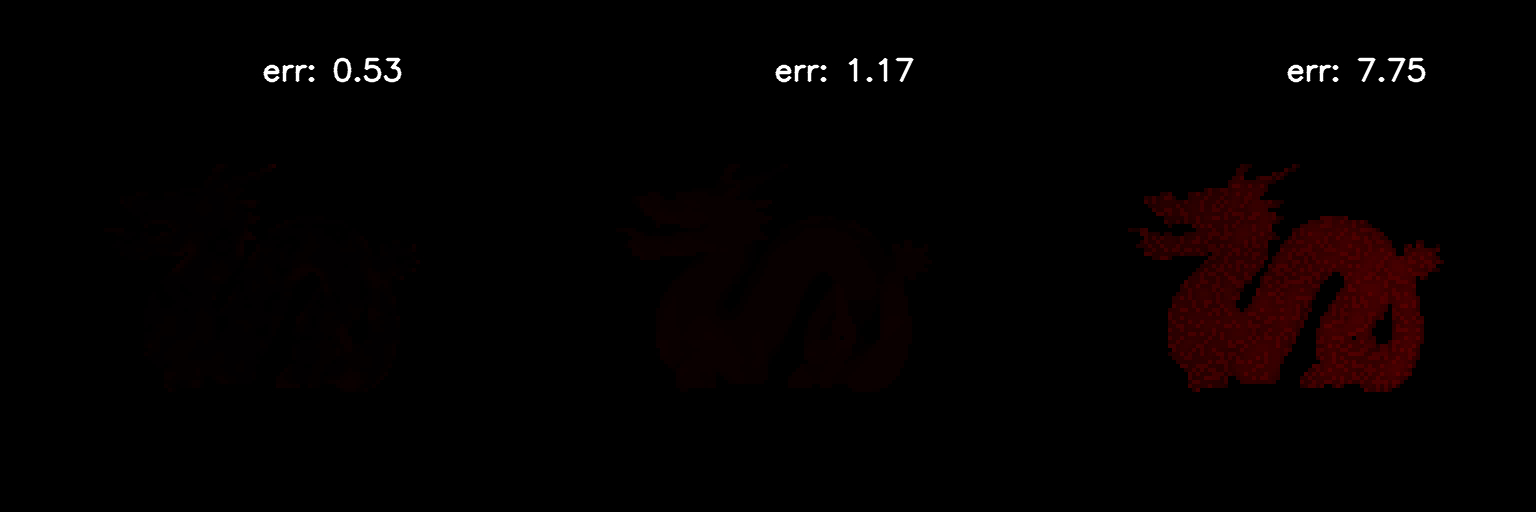
\includegraphics[width=0.18\linewidth]{./Figures/light-synthetic/fancy_eval_1_output_error.png}
	
	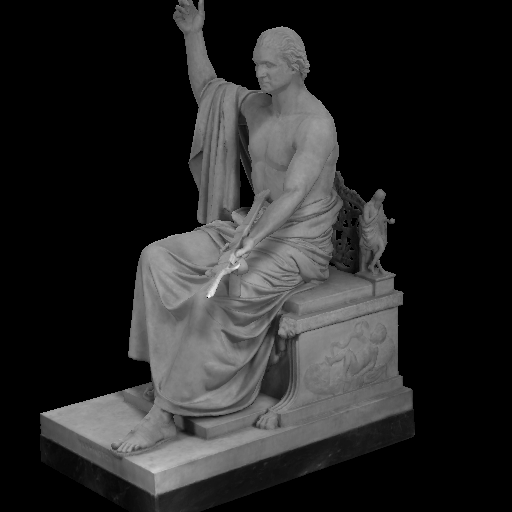
\includegraphics[width=0.18\linewidth]{./Figures/light-synthetic/fancy_eval_4_img.png}
	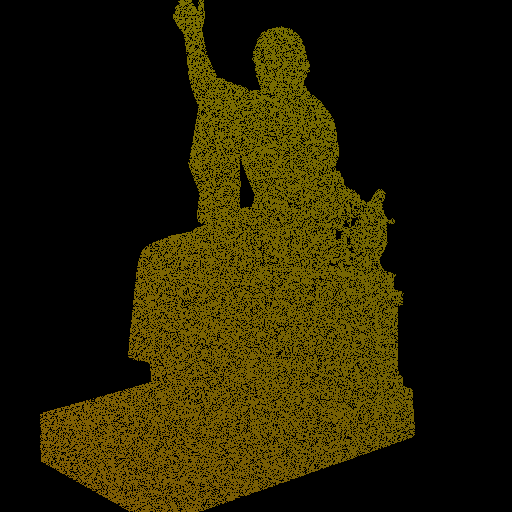
\includegraphics[width=0.18\linewidth]{./Figures/light-synthetic/fancy_eval_4_light_input.png}
	
\includegraphics[width=0.18\linewidth]{./Figures/light-synthetic/fancy_eval_4_light_light.png}
	
\includegraphics[width=0.18\linewidth]{./Figures/light-synthetic/fancy_eval_4_light_gt.png}
	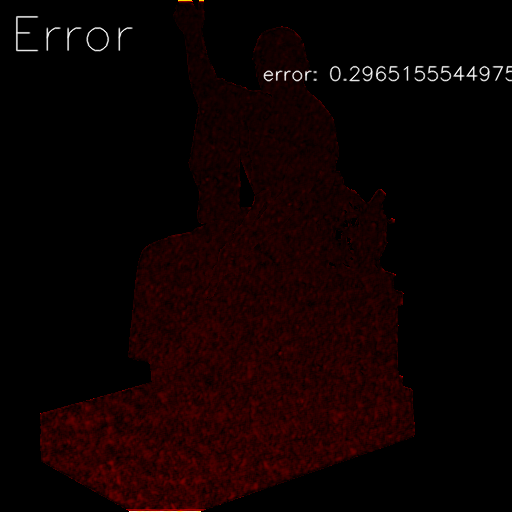
\includegraphics[width=0.18\linewidth]{./Figures/light-synthetic/fancy_eval_4_output_error.png}
	
	\caption{Qualitative evaluation of light net on Sphere, bus and Washington statue. From left to right, grayscale image, semi-dense light map(input), full-dense light map(output), full-dense light map(ground-truth), error map.}
	\label{fig:eval-light}
\end{figure}

Figure \ref{fig:scatter-light} uses a scatter plot to show the average angular error on 100 different test cases. The average pixel-wise angular error is 0.17 degree as shown in Table \ref{tab:model-error}. An regression line has been added in the plot to analysis the tendency of the errors. The angular error slightly goes up when valid point number in the scene increase. It is make sense since the valid pixels are usually connected and concentrate in a single patch, the less of the area of the patch, which corresponding the number of the valid points, the less variation of the light direction among the pixels, thus better the evaluation.


\begin{figure}[th]
	\centering
	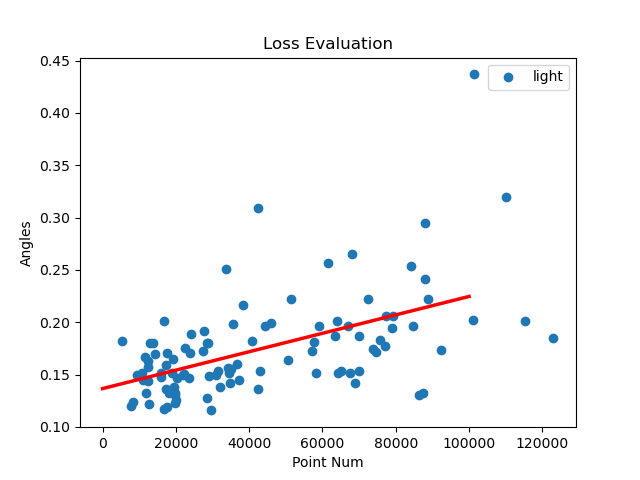
\includegraphics[width=0.5\linewidth]{./Figures/scatter-light-noised.png}
	\caption{The evaluation on 100 test cases of Light Net.}
	\label{fig:scatter-light}
\end{figure}



\subsection{Trignet Net Evaluation}


The qualitative evaluation of Trignet uses the model trained based on masked L2 loss.

\subsubsection{title}

\begin{figure}[th]
	\centering
	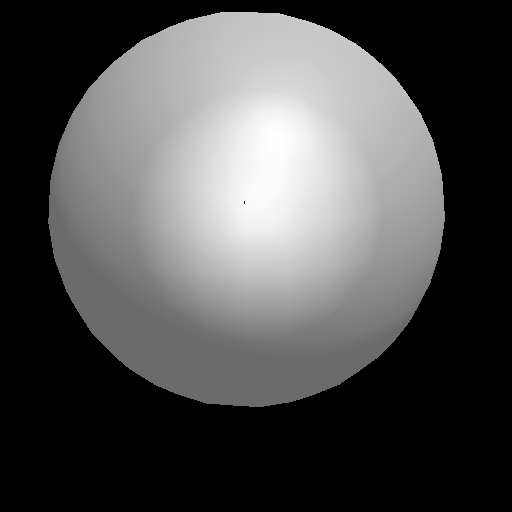
\includegraphics[width=0.18\linewidth]{./Figures/light-synthetic/fancy_eval_0_img.png}
	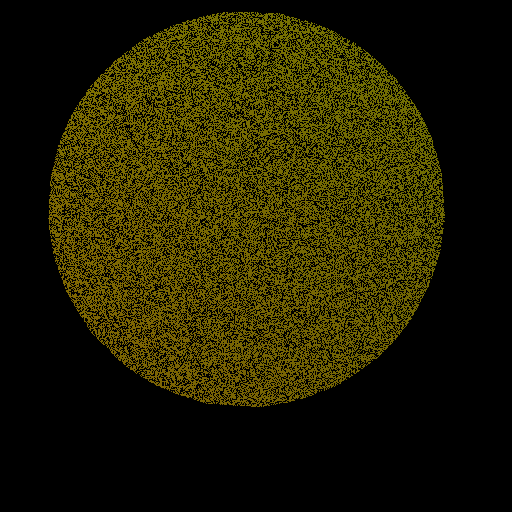
\includegraphics[width=0.18\linewidth]{./Figures/light-synthetic/fancy_eval_0_light_input.png}
	
\includegraphics[width=0.18\linewidth]{./Figures/light-synthetic/fancy_eval_0_light_light.png}
	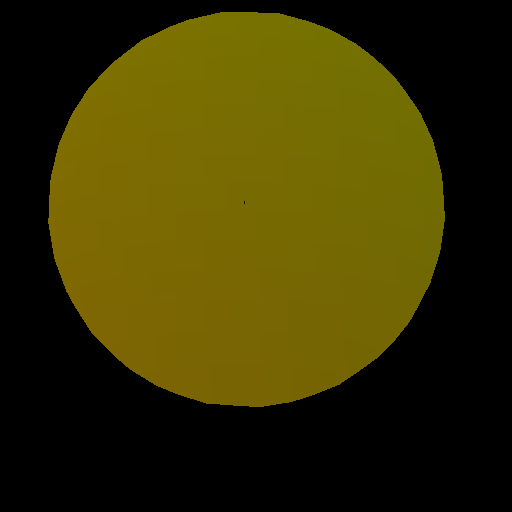
\includegraphics[width=0.18\linewidth]{./Figures/light-synthetic/fancy_eval_0_light_gt.png}
	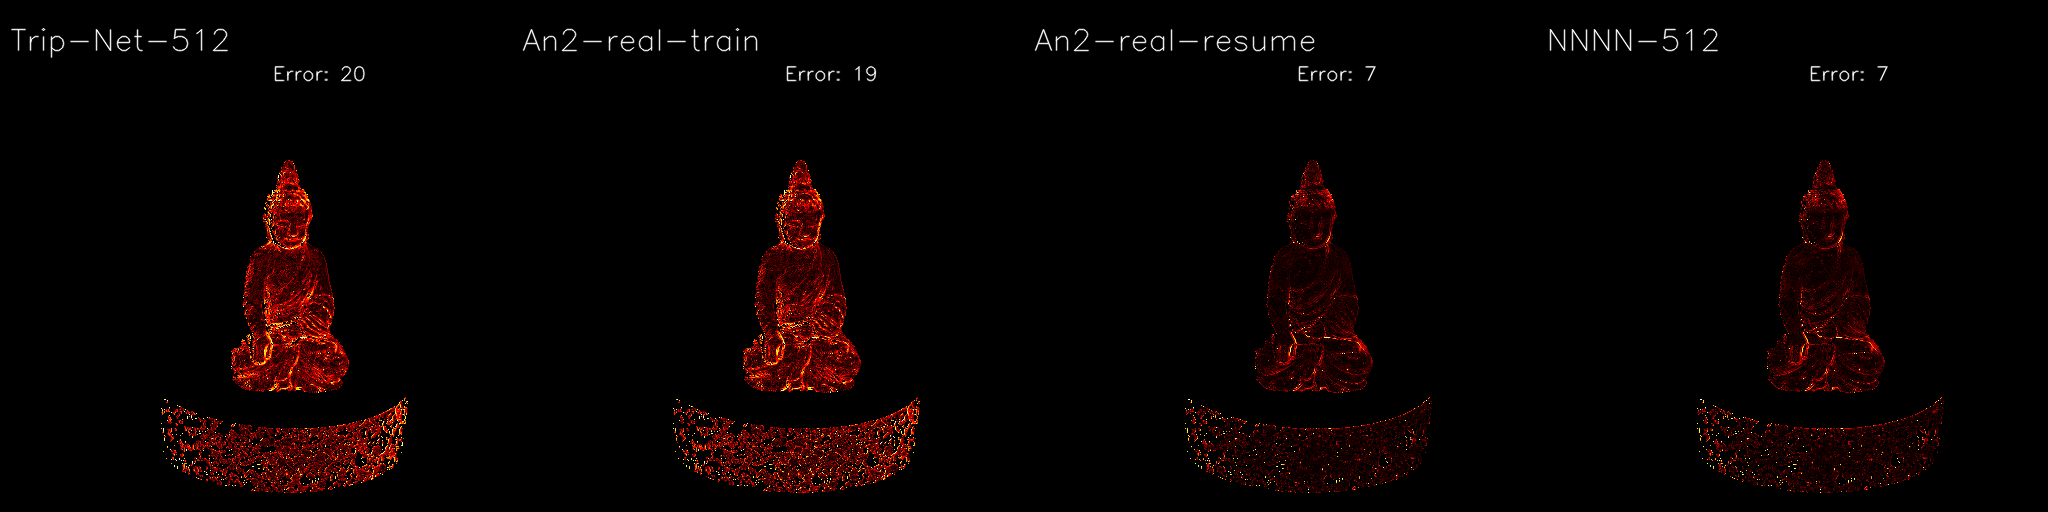
\includegraphics[width=0.18\linewidth]{./Figures/light-synthetic/fancy_eval_0_output_error.png}
	
	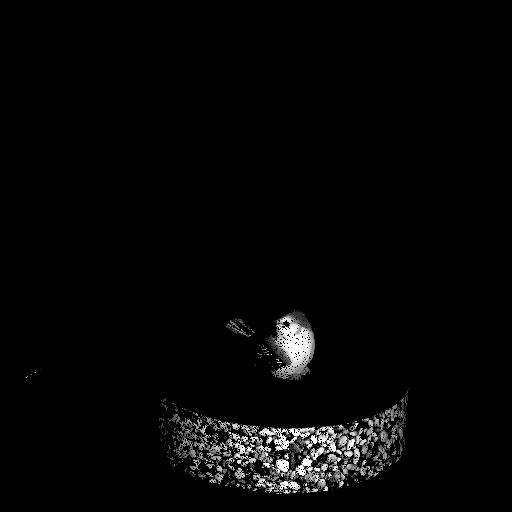
\includegraphics[width=0.18\linewidth]{./Figures/light-synthetic/fancy_eval_1_img.png}
	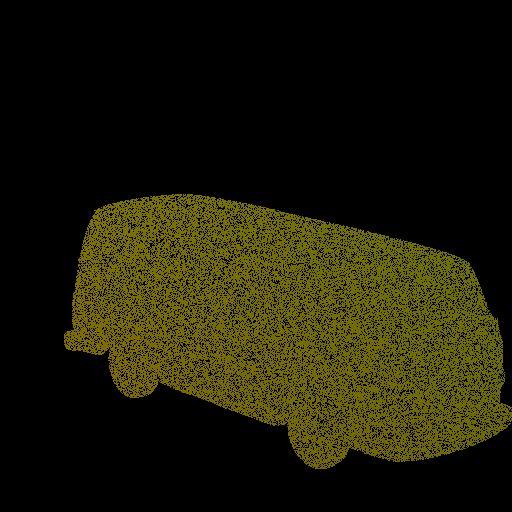
\includegraphics[width=0.18\linewidth]{./Figures/light-synthetic/fancy_eval_1_light_input.png}
	
\includegraphics[width=0.18\linewidth]{./Figures/light-synthetic/fancy_eval_1_light_light.png}
	
\includegraphics[width=0.18\linewidth]{./Figures/light-synthetic/fancy_eval_1_light_gt.png}
	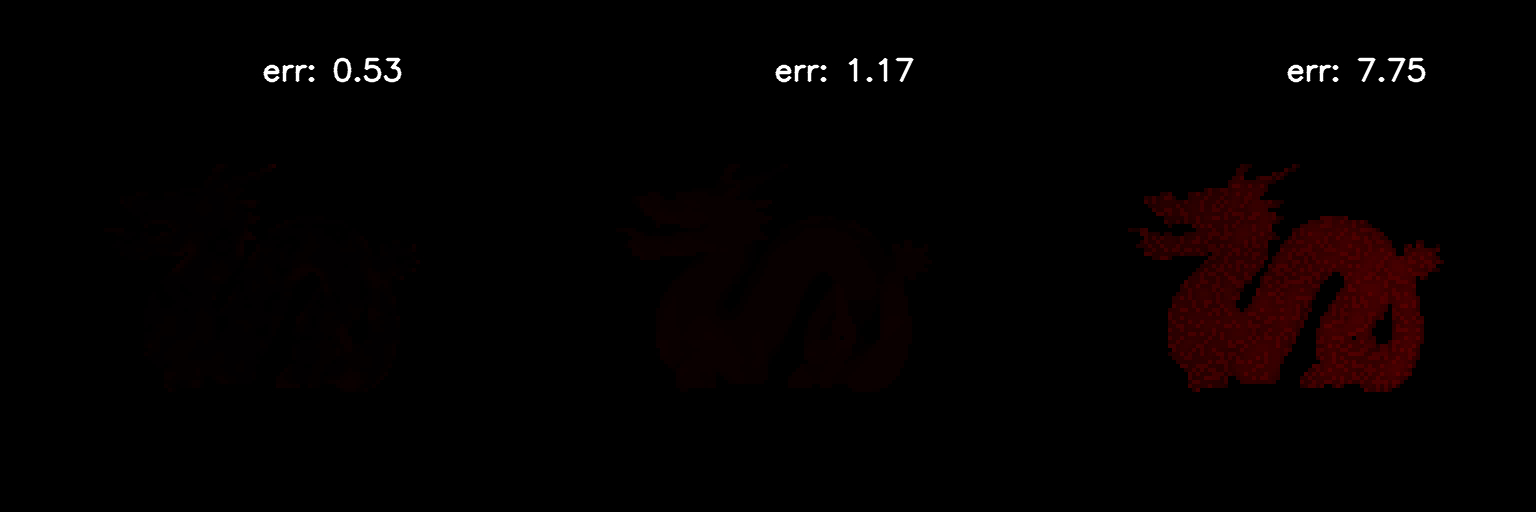
\includegraphics[width=0.18\linewidth]{./Figures/light-synthetic/fancy_eval_1_output_error.png}
	
	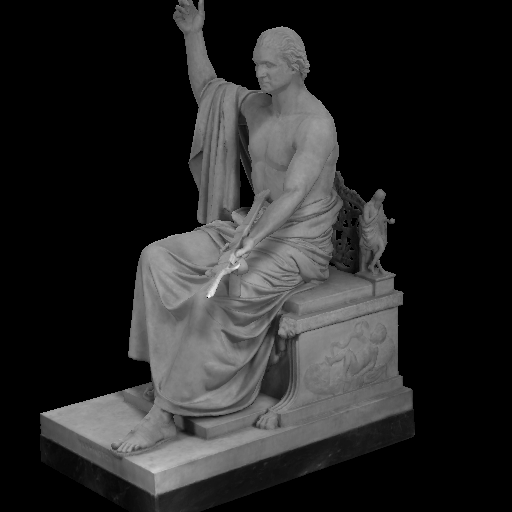
\includegraphics[width=0.18\linewidth]{./Figures/light-synthetic/fancy_eval_4_img.png}
	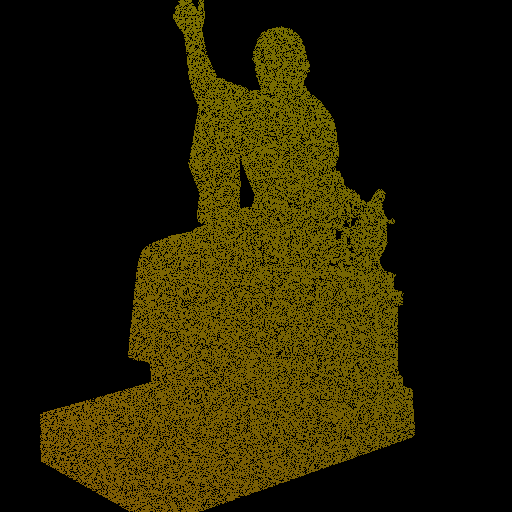
\includegraphics[width=0.18\linewidth]{./Figures/light-synthetic/fancy_eval_4_light_input.png}
	
\includegraphics[width=0.18\linewidth]{./Figures/light-synthetic/fancy_eval_4_light_light.png}
	
\includegraphics[width=0.18\linewidth]{./Figures/light-synthetic/fancy_eval_4_light_gt.png}
	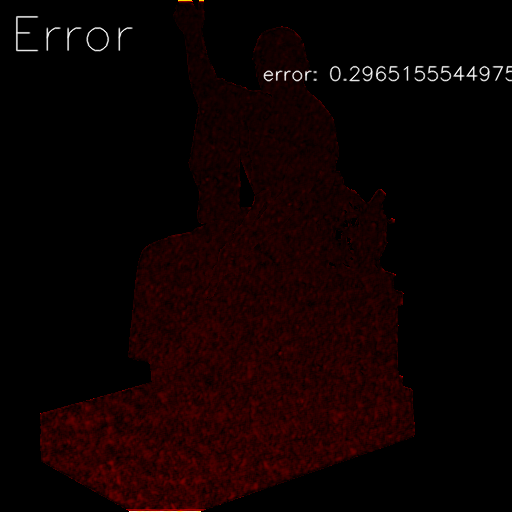
\includegraphics[width=0.18\linewidth]{./Figures/light-synthetic/fancy_eval_4_output_error.png}
	
	\caption{Qualitative evaluation of Trignet net on Sphere, bus and Washington statue. From left to right, semi 3D vertex map, full-dense normal map(output), full-dense normal map(ground-truth), error map.}
	\label{fig:eval-trignet}
\end{figure}

\begin{figure}[th]
	\centering
	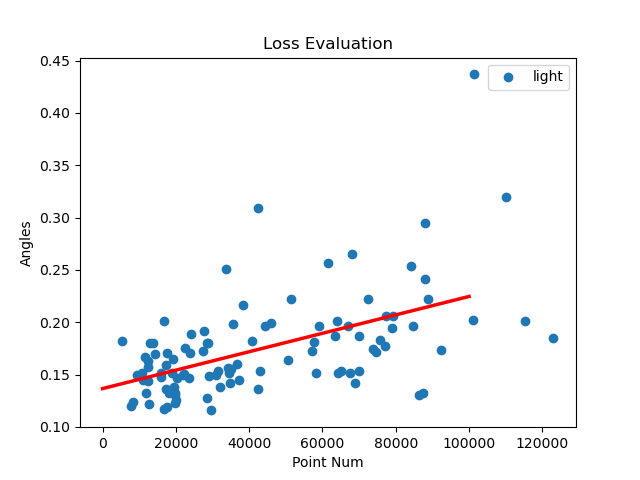
\includegraphics[width=0.5\linewidth]{./Figures/scatter-light-noised.png}
	\caption{The evaluation on 100 test cases of Trignet.}
	\label{fig:scatter-trignet}
\end{figure}




\subsection{comparison}
From the Figure \ref{fig:normal-histo-diff} we can observe the normal difference between ground-truth and GCNN predicted normals in another dimension. It separates the interval $ \left[ -1,1 \right] $, which is exactly the range of normal vector, to 256 sections. Then it counts the number of points locates in each section for 3 axes.  The 3 axes are fitted quite well in most of interval but other than $ \left[ -0.25,0.25 \right] $ for x and y axes and  interval close to $ -1 $ for z axis. Therefore a further constraint can be considered to the loss function related to the normal difference shown in this figure.

It is faulty that almost no normal has -1 z-component in GCNN predicted normal map. The reason?
\begin{figure}[th]
	\centering
	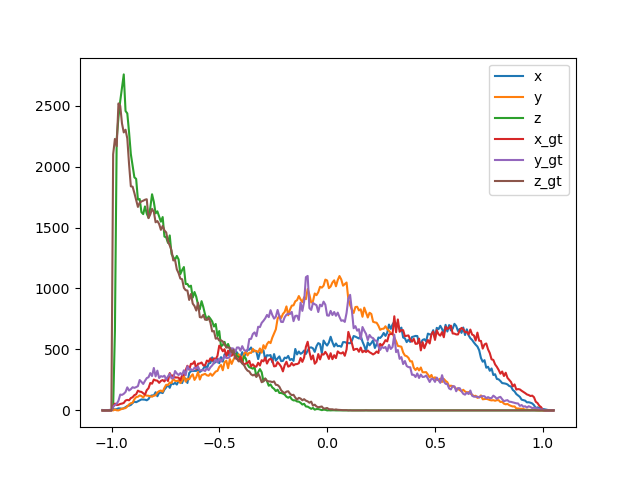
\includegraphics[width=\linewidth]{./Figures/normal-histo-diff.png}
	\caption{The normal difference of between GCNN and ground-truth in x, y, z-axis respectively. The y axis indicates the number of points, x axis indicates the value of normal in x/y/z axis. (The chart is based on the "dragon" scene showing above)}
	\label{fig:normal-histo-diff}
\end{figure}
	

\begin{table}[th]
	
	\centering
	\begin{tabular}{l l l l l l l }
		\toprule
		\tabhead{Model} & \tabhead{Angle} & \tabhead{Time /ms} & \tabhead{bz} & \tabhead{lr-schedule} & \tabhead{lr-df} & \tabhead{l/i. Nr.}\\
		\midrule
		LightNet  & 0.17  & 4.72 & &  & &\\ 
		\hline
		GCNN  & 10.57 & 5.25 & 8 & 200,1600 & 0.5 & 0 \\
		\hline
		an3 & 9999 & 9999 & 8 &  & & 1\\
		\hline
		VIL-1 & 10.64 & 31.57 & 8 & 10,1000 & 0.5 & 1\\
		\hline
		VIL-1 & 10.87 & 32.61 & 8 & 3,12,1000 & 0.5 & 1\\
		\hline
		VIL-3  & 10.83 & 53.95 & 8 & 100,1000 & 0.1 & 3\\
		\hline
		VIL-10  & 11.20 & 134.28 & 8 & 100,1000 & 0.1 &10\\
		\bottomrule\\
	\end{tabular}
	\caption{The error of models. The angle error is the average angle error of all valid pixels in the test case. The time unit is millisecond. bz is the batch size, lr-schedule is learning rate schedule. lr-df is learning rate decay factor, l/i. Nr is the number of light-image maps used for each scene}	
	\label{tab:model-error}
\end{table}


\begin{figure}[th]
	\centering
	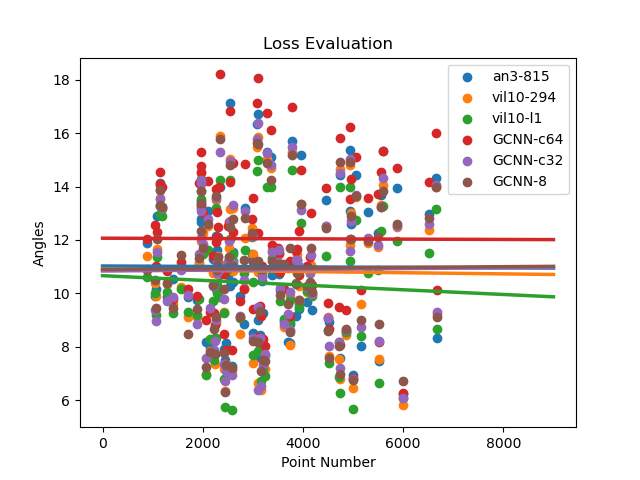
\includegraphics[width=\linewidth]{./Figures/regression-comparison.png}
	\caption{The normal difference of between GCNN and ground-truth in x, y, z-axis respectively. The y axis indicates the number of points, x axis indicates the value of normal in x/y/z axis. (The chart is based on the "dragon" scene showing above)}
	\label{fig:normal-histo-diff}
\end{figure}

\end{document}
